\documentclass[../main.tex]{subfiles}

\begin{document}

\section{Setting up the CTF environment}

In this section, we will quickly go over our choice of CTF environment and how to set it up in Google Cloud. The CTF environment, we decided to use was CTFd. CTFd is a CTF platform solution that is free and open-source and can be hosted on any machine of your choosing. They also offer a SaaS hosted solution on their website, but this was too expensive for us. We don't actually need a professionally hosted service for this project anyways. Our CTF environment will most likely never be used by more than a few people at once. This means that our installation could be done in a fairly basic way, without any automatic scaling or other such extras needed.

\subsection{Google Cloud script}

We wanted to keep the deployment of our application simple and to the point. For this reason, we decided to use a small deployment script alongside Docker to start up our VM and the CTFd service.

The deployment script we wrote is small and can initialize and delete our Gcloud virtual machines. This is done through two command line options: \lstinline{-i} to create and initialize (install and start Docker) the machine in Gcloud, and \lstinline{-r} to remove the running machine. This is done by using a simple \lstinline{test} expression:

\begin{lstlisting}
[ "$1" = "-i" ] && install
[ "$1" = "-r" ] && remove
[ -z "$1" ] && printhelp && exit 0
\end{lstlisting}

The source code for the script can be found on our GitHub organization\footnote{\url{https://github.com/kdg-cybersecurity-gr5}} under the \lstinline{deployment} repository.

When initializing the machine, it gets coupled to an existing external IP that we linked to our domain name, \lstinline{verkiezingen.xyz}. This external IP address doesn't get removed by the \lstinline{-r} command because if it did, we would have to set up our DNS records every time we restarted our machine. Keeping the IP active like this when there is no machine attached does cost money\footnote{\url{https://cloud.google.com/vpc/network-pricing\#ipaddress}}, but we have enough credits to last us until the end of the project so this will not be an issue for us.

\subsection{Docker run scripts}

To run our application we use Docker containers started with the \lstinline{docker run} command on our Gcloud virtual machines. This command is found in the \lstinline{run.sh} file located in our \lstinline{deployment} repository. The \lstinline{run.sh} file gets invoked by our previously mentioned Gcloud deployment script after it boots up the machine itself.

Alongside our application, we also start a Traefik container to help route the traffic to an HTTPS environment as well as provide a signed certificate for our application using LetsEncrypt. This container is set up to accept connections from the ports 80 and 443. It routes all requests made to \lstinline{ctf.verkiezingen.xyz} to our application in the same Docker network. By doing this we don't need to expose our application directly to the internet, thus providing ourselves with added security.

We also reuse this Traefik container later to route our web challenges to the right place. By doing this, we can put all of our challenges on a subdomain of \lstinline{verkiezingen.xyz}. This alongside the HTTPS provided gives an added layer of authenticity.

\subsection{CTFd initial setup}

Settings up CTFd is quite simple, and we won't go into much detail here. We followed the setup instructions and changed our title and description.

\subsubsection{Theming}

We set out to personalize our CTF environment using a United States theme\footnote{\url{https://github.com/ColdHeat/UnitedStates}}. It turned out however that this theme is either outdated in some way or it's just broken. We tried multiple ways to get it installed, to no avail. Each time we turned to the theme, the whole site would look broken.

This means we had to settle for theming our environment using the favicon and logo. Here we decided to use the United States flag, as per our subject matter.

\newpage

\subsubsection{Setup complete}

Our setup of the CTFd environment is now complete and looks like this.

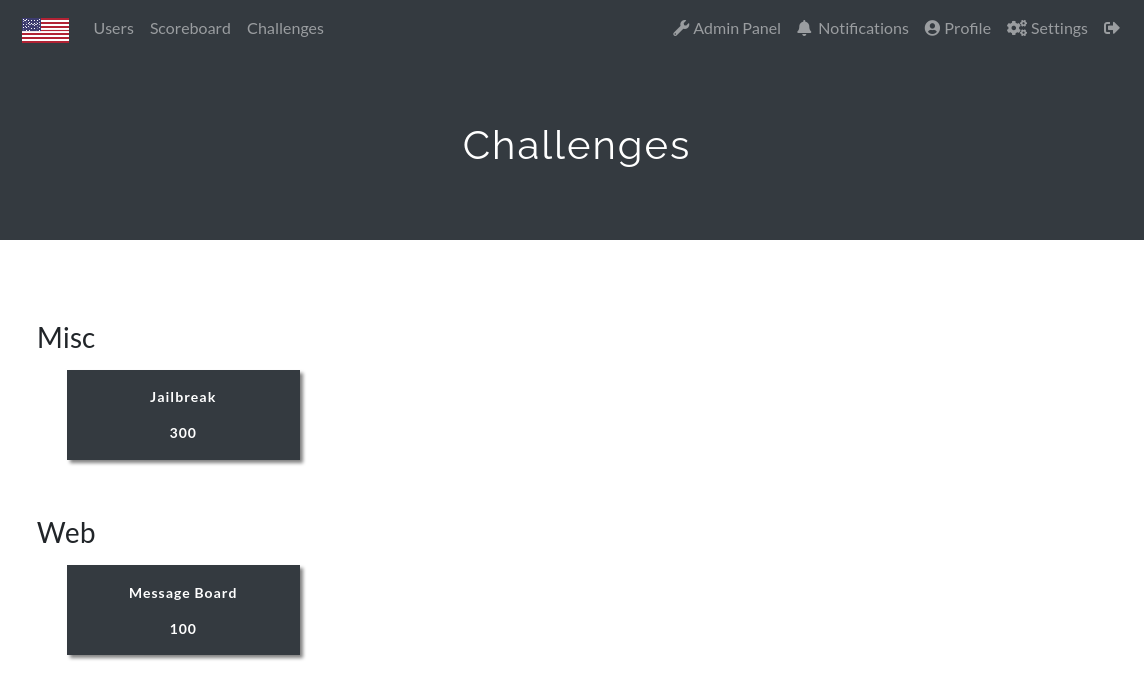
\includegraphics[width=\linewidth]{images/ctfd.png}

Everyone can now add their challenges using admin credentials. New users can register on our platform without needing an admin's help.



\end{document}
